\section{实验}

\begin{figure*}[t]
  \centering
  \vspace{0.5em}
  \begin{minipage}[t]{0.66\textwidth}
    \vspace{0pt}
    \centering
    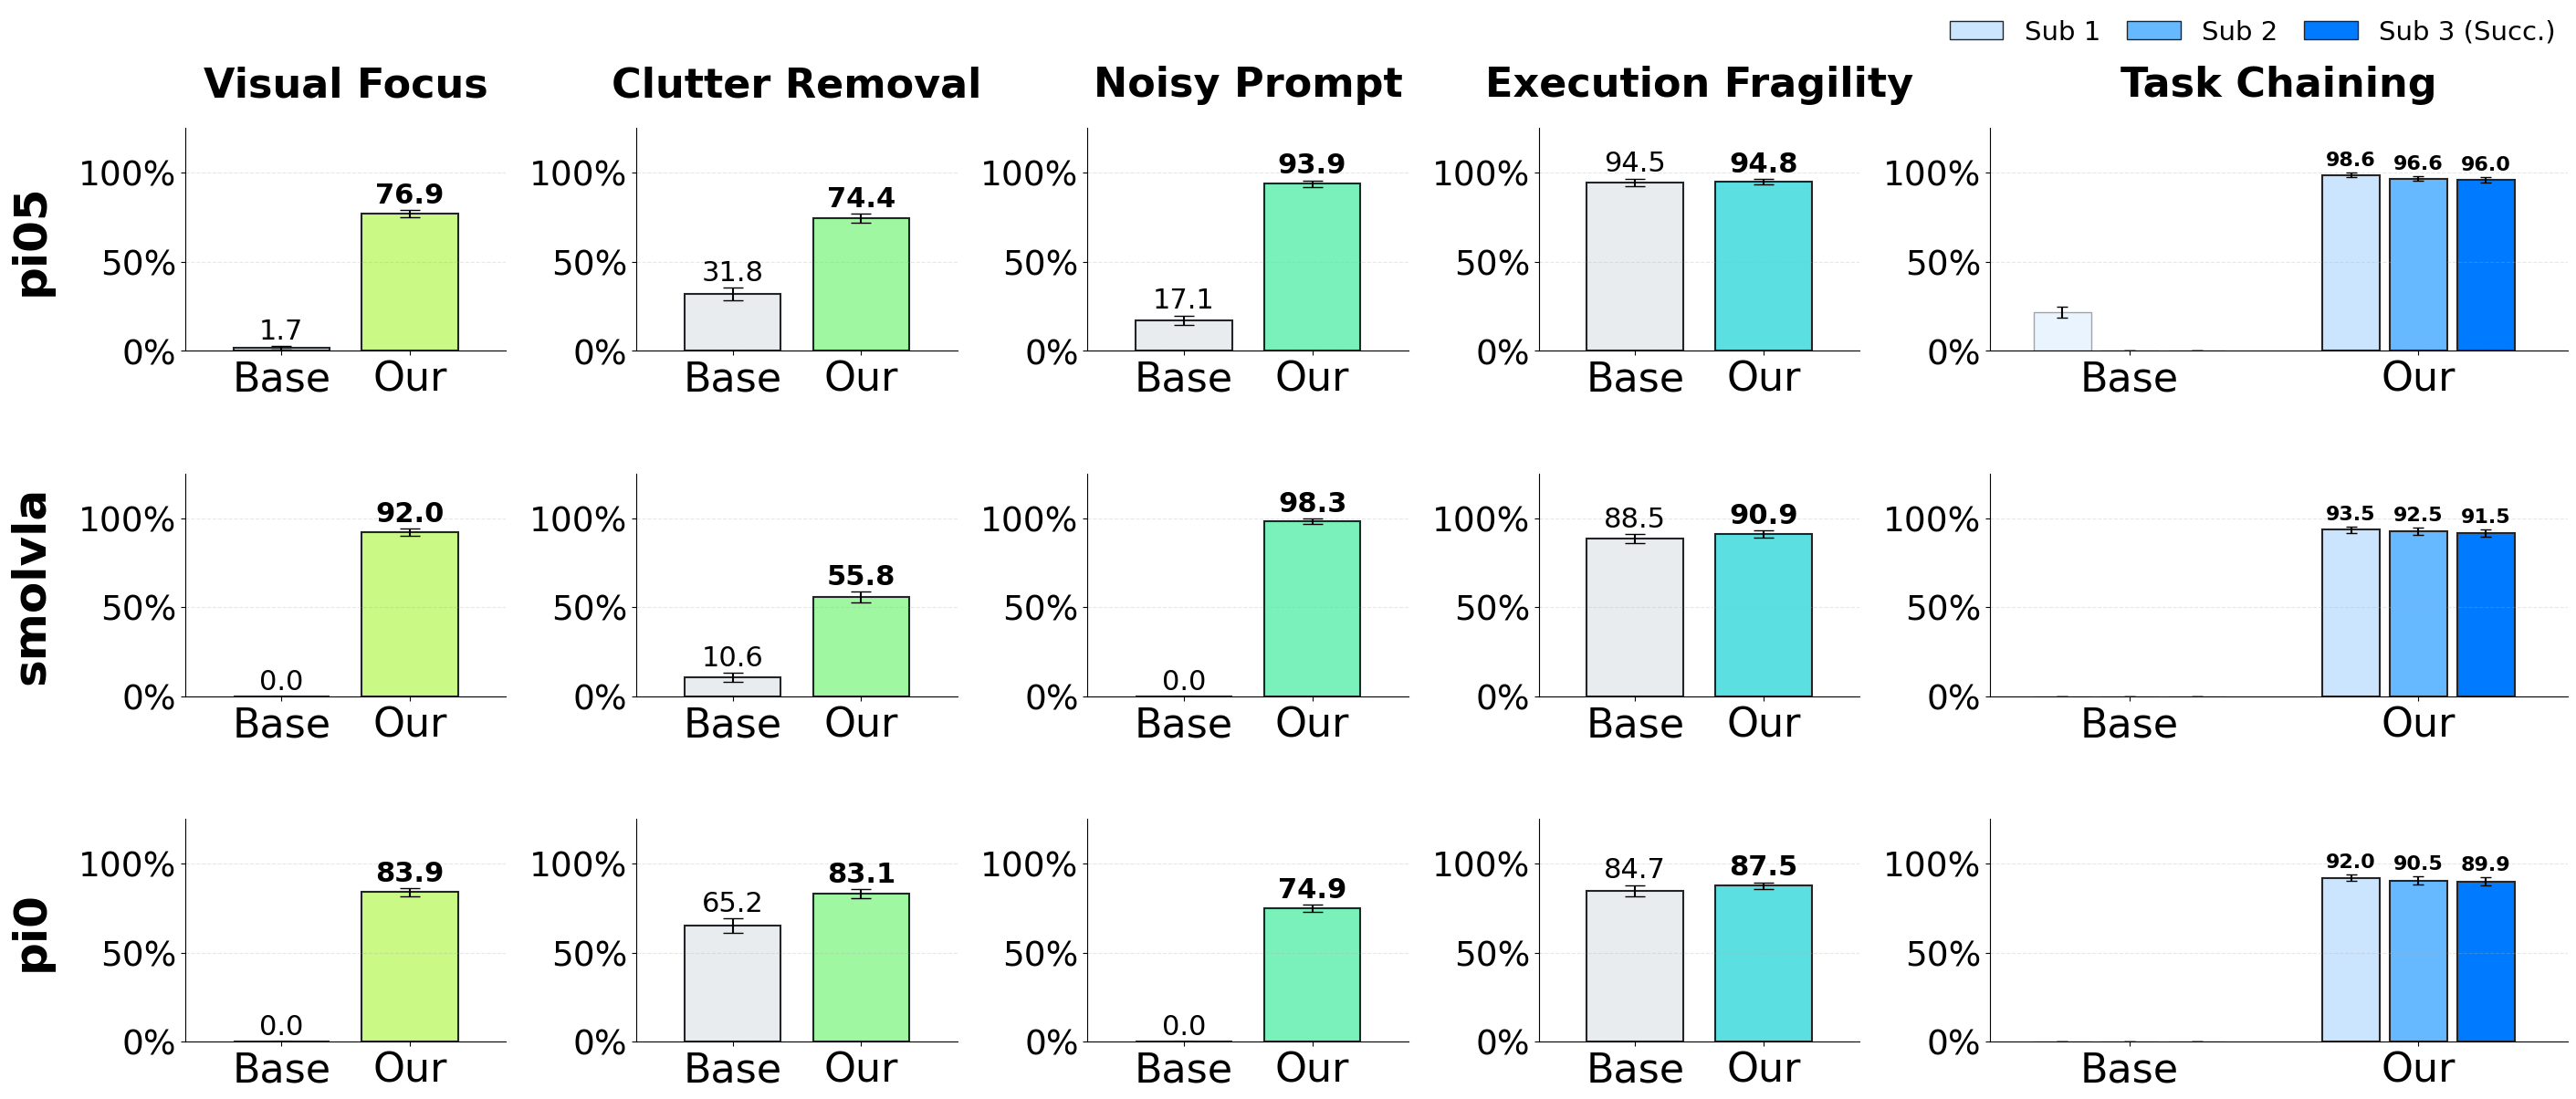
\includegraphics[width=\linewidth]{figure/result.png}
    \captionof{figure}{\textbf{LIBERO-\sys\ 上的性能。}比较 \sys\ 与 VLA 基线在视觉、语言和长时程挑战上的表现。}
    \label{fig:result}
  \end{minipage}%
  \hspace{0.01\textwidth}%
  \begin{minipage}[t]{0.30\textwidth}
    \vspace{0pt}
    \centering
    {\color{black}
    \vspace{0pt}
    \small
    \setlength{\tabcolsep}{3pt}
    \renewcommand{\arraystretch}{1.02}
    \begin{tabular}{@{}p{0.48\linewidth}lr@{}}
    \toprule
    \multicolumn{1}{@{}l}{\textbf{组件}} & & \textbf{ms/步} \\
    \midrule
    \multirow{2}{=}{基线 rollout} & 均值 & 15.31 \\
    & P95 & 15.98 \\
    \cmidrule(lr){1-3}
    \multirow{2}{=}{RAG 检索} & 均值 & 0.005 \\
    & P95 & 0.005 \\
    \cmidrule(lr){1-3}
    \multirow{2}{=}{VLM 编排} & 均值 & 7.20 \\
    & P95 & 8.65 \\
    \cmidrule(lr){1-3}
    \multirow{2}{=}{SAM3 + 叠加} & 均值 & 0.16 \\
    & P95 & 0.16 \\
    \cmidrule(lr){1-3}
    \multirow{2}{=}{SAM3 + 移除} & 均值 & 0.16 \\
    & P95 & 0.16 \\
    \bottomrule
    \end{tabular}
    \vspace{-0.3em}
    \captionsetup{justification=raggedright,singlelinecheck=false}
    \vspace{0.2em}
    \captionof{table}{\textbf{运行时开销。}在 1000 个 LIBERO 步上摊销。}
    \label{tab:runtime_overhead}
    \renewcommand{\arraystretch}{1.0}
    }
  \end{minipage}
  \vspace{-0.5em}
\end{figure*}

\begin{table}[t]
  \centering
  \caption{\textbf{LIBERO-PRO 上的性能。}布局（Pos）和语义（Task）偏移下的成功率。}
  \label{tab:libero_pro}
  \small
  \addtolength{\tabcolsep}{-4pt}
  {
  \setlength{\aboverulesep}{0pt}
  \setlength{\belowrulesep}{0pt}
  \begin{tabular}{l|clcc}
    \toprule
    \rule{0pt}{3ex} \textbf{层级} & \textbf{类别} & \textbf{任务（符号形式）} & \textbf{$\pi_{0.5}$基线} & \textbf{使用本文方法} \\
    \midrule
    \rule{0pt}{2.5ex} \multirow{6}{*}{\textbf{Pos}} & \multirow{5}{*}{\textbf{空间}}
      & $P.(btw(p, r), pl.)$         & 2\%  & \textbf{63.0\%} \\
    & & $P.(center, pl.)$             & 0\%  & \textbf{97.0\%} \\
    & & $P.(drw_{top}(cab_{w}), pl.)$ & 0\%  & \textbf{20.2\%} \\
    & & $P.(next\_to(p), pl.)$        & 0\%  & \textbf{57.0\%} \\
    & & $P.(next\_to(r), pl.)$        & 12\% & \textbf{71.0\%} \\
    \cmidrule(l){2-5}
    & \rule{0pt}{2.5ex} \textbf{物体} & $P.(soup, bskt.)$ & 0\% & \textbf{35.0\%} \\
    \midrule
    \multicolumn{3}{l|}{\rule{0pt}{2.5ex} \textit{\textbf{平均值（Pos）}}} & 2.33\% & \textbf{57.2\%} \\
    \midrule
    \rule{0pt}{3ex} \multirow{14}{*}{\textbf{Task}} & \multirow{9}{*}{\textbf{空间}}
      & $P.(btw(p, r), pl.)$       & 0\% & \textbf{78.0\%} \\
    & & $P.(center, pl.)$           & 2\% & \textbf{82.0\%} \\
    & & $P.(next\_to(ck.), pl.)$    & 2\% & \textbf{97.0\%} \\
    & & $P.(next\_to(p), pl.)$     & 0\% & \textbf{73.0\%} \\
    & & $P.(next\_to(r), pl.)$     & 2\% & \textbf{98.0\%} \\
    & & $P.(on(ck.), pl.)$          & 0\% & \textbf{12.0\%} \\
    & & $P.(on(r), pl.)$            & 2\% & \textbf{100.0\%} \\
    & & $P.(on(stove), pl.)$        & 0\% & \textbf{13.0\%} \\
    & & $P.(on(cab_{w}), pl.)$      & 0\% & \textbf{95.0\%} \\
    \cmidrule(l){2-5}
    & \rule{0pt}{2.5ex} \multirow{5}{*}{\textbf{物体}}
      & $P.(soup, bskt.)$           & 0\% & \textbf{16.0\%} \\
    & & $P.(bbq, bskt.)$            & 2\% & \textbf{32.0\%} \\
    & & $P.(juice, bskt.)$          & 2\% & \textbf{41.0\%} \\
    & & $P.(dressing, bskt.)$       & 0\% & \textbf{13.0\%} \\
    & & $P.(tomato, bskt.)$         & 0\% & \textbf{23.0\%} \\
    \midrule
    \multicolumn{3}{l|}{\rule{0pt}{2.5ex} \textit{\textbf{平均值（Task）}}} & 0.86\% & \textbf{55.2\%} \\
    \bottomrule
  \end{tabular}
  }
  \vspace{-1.5em}
\end{table}

我们在 25 项任务上，使用多个基础模型评估 \sys，并进一步通过消融实验验证双阶段记忆巩固机制。
结果表明，\sys\ 在不同场景下均能持续改善上下文内自适应和策略鲁棒性。

为在真实机器人实验成本和试验次数约束下提高统计可靠性，我们优先在高保真仿真环境中进行严格测试。

\subsection{实验设置}

\noindent\textbf{任务设计与评估基准。}
为评估分布偏移下的鲁棒上下文内自适应，我们在两个任务套件上进行实验。
首先采用 \textbf{LIBERO-PRO}~\cite{liberopro} 基准，测试空间和物体类别中位置交换（LIBERO-PRO Pos）与任务级变化（LIBERO-PRO Task）下的鲁棒性。

此外，我们提出 \textbf{LIBERO-\sys}。
该套件在仿真和真实机器人场景中形式化了五类\textit{常见且关键}的 OOD 挑战维度。
它通过重新配置 LIBERO 场景~\cite{libero_ref}中的资产，提供一个受控环境，用于评估智能体无需任务特定微调、针对反复出现的失败模式触发自适应干预的能力。

\begin{itemize}
    \item \textbf{视觉聚焦：}从五个外观相同的新碗中选择目标。我们用不可区分的资产替换 \textit{LIBERO-Spatial} 目标，以评估细粒度视觉歧义下的\textbf{指称落地}。

    \item \textbf{杂物移除：}在密集干扰物中抓取目标。我们在 \textit{LIBERO-Spatial} 中加入高熵物体簇，以测试拥挤场景中的\textbf{操作聚焦}和干扰缓解能力。

    \item \textbf{噪声提示：}从措辞或任务结构偏离历史成功经验模式的指令中提取意图（例如“呃……拿那个红色、捏起来软软的东西”）。我们向 \textit{LIBERO-Object} 指令注入语言噪声，以评估\textbf{语言鲁棒性}和\textbf{以经验为落地依据的语义映射}。

    \item \textbf{执行脆弱性：}细微滑动便会导致失败的关键操作。我们从 \textit{LIBERO-Object} 中整理不稳定子任务，以评估面对机械不确定性时的\textbf{操作稳定性}。

    \item \textbf{任务串联：}将多个物体分拣到篮子中的长时程任务。该任务通过串联原子的 \textit{LIBERO-Object} 动作，评估顺序工作流中的\textbf{长期推理}和\textbf{错误韧性}。
\end{itemize}

\noindent\textbf{上下文内初始化与指标。}
我们首先在标准 LIBERO-Object 和 LIBERO-Spatial 集上执行一次初步推理，以初始化双记忆 RAG。
这种非参数“冷启动”会用通用执行轨迹填充记忆库，但不进行基于梯度的训练，也不会接触评估时的 OOD 扰动。
随后，我们对每项任务运行 199 次随机化 rollout，充分打乱物体位姿和任务序列以减少偏差。
性能以\textbf{总体完成率}和\textbf{中间成功率}衡量，后者用于细粒度分析长时程任务。

\noindent\textbf{基线。}
我们在多种基础模型上评估 \sys，包括 $\pi_0$~\cite{pi0}、$\pi_{0.5}$~\cite{pi05} 和 SmolVLA~\cite{SmolVLA}。
在各 OOD 场景中，\sys\ 均持续提高成功率，表明策略泛化能力得到改善。

\subsection{主要结果}
\label{Main Results}

如图~\ref{fig:result} 和表~\ref{tab:libero_pro} 所示，\sys\ 增强的策略在 LIBERO-\sys\ 与 LIBERO-PRO 上均提高了鲁棒性，尤其是在感知歧义、语言噪声和长时程误差复合的情况下。

\subsubsection{LIBERO-\sys\ 上的结果}

\noindent\textbf{环境与语言变化。}
基础模型对感知和语言干扰十分敏感。
对于 \textit{pi05-LIBERO}，使用 \sys\ 后，\textit{视觉聚焦}和\textit{杂物移除}的成功率分别从 $1.7\%$ 和 $31.8\%$ 提升至 $76.9\%$ 和 $74.4\%$，说明基于 MCP 的干预有助于隔离与任务相关的物体。
对于语言扰动，\textit{smolvla-LIBERO} 经指令改写后在\textit{噪声提示}上的成功率达到 $98.3\%$。

\noindent\textbf{执行稳定性与长时程任务。}
在\textit{执行脆弱性}任务中，\sys\ 通过加入面向恢复的干预，使所有模型的成功率都提高到 $87\%$ 以上。
由于\textit{执行脆弱性}的基线成功率本来就相对较高，\sys\ 的绝对提升较小，主要通过回滚和重试减少剩余的少数失败。
在\textit{任务串联}中，\sys\ 通过子任务分解与控制流重置减少复合误差；值得注意的是，\textit{pi05-LIBERO} 到最后一个子任务仍保持 $96.0\%$ 的成功率。

\subsubsection{LIBERO-PRO 上的结果}

\noindent\textbf{位置级布局偏移。}
在 LIBERO-PRO Pos 下，$\pi_{0.5}$ 基线平均成功率仅为 $2.33\%$，而 \sys\ 将其提高到 $57.2\%$。
这表明记忆引导的视觉干预有助于在布局偏移下恢复物体落地。

\noindent\textbf{任务级语义扰动。}
在 LIBERO-PRO Task 下，基线平均成功率仅为 $0.86\%$，而 \sys\ 达到 $55.2\%$。
这些提升说明 \sys\ 改善了冻结控制器的输入和任务上下文，而不是替代底层 VLA 策略。

\subsubsection{讨论}
这些大幅提升源于对冻结 VLA 在 OOD 布局、干扰物、噪声提示和长时程链中无状态特性的补偿。
\sys\ 检索成功/失败记忆以诊断失败，并在执行前触发任务级 MCP 干预。

\subsubsection{在线延迟}
表~\ref{tab:runtime_overhead} 报告了在一个 1000 步 LIBERO 任务上摊销的延迟，其中基线 rollout 在 RTX 4090 上测得。
RAG 检索和基于 SAM3 的工具只增加可忽略的摊销开销，VLM 编排则是主要的额外成本。
由于 \sys\ 在 rollout 之前、而非每个策略步都调用这些模块，底层执行仍然流畅且非阻塞。
在流水线化的多任务设置中，下一项任务的编排可以与当前任务的执行重叠。

\subsection{消融实验}

在第~\ref{Main Results} 节验证编排器与 MCP 模块之后，我们进一步分析双记忆 RAG 系统的\textbf{双重}设计。
我们分两步进行：先分离双记忆库对执行效率的影响，再评估双阶段记忆巩固对推理深度的贡献。

\subsubsection{双记忆库的有效性}
\label{dual memory ablation}

为验证成功与失败经验在锚定编排器决策时都不可或缺，我们采用平均成功轮数（Average Turns-to-Success）~\cite{multiwoz,toolsandbox}，即达到最优方案所需的推理--干预循环次数。
当一次干预失败时，智能体会得到稀疏的环境反馈，并必须在后续轮次中自我纠正。
如图~\ref{fig:ablation_beeswarm} 所示，我们比较四种记忆配置：\textbf{无记忆}、\textbf{仅失败}、\textbf{仅成功}以及\textbf{\sys（双记忆）}。

\begin{figure}[htbp]
   \vspace{0.5em}
    \centering
    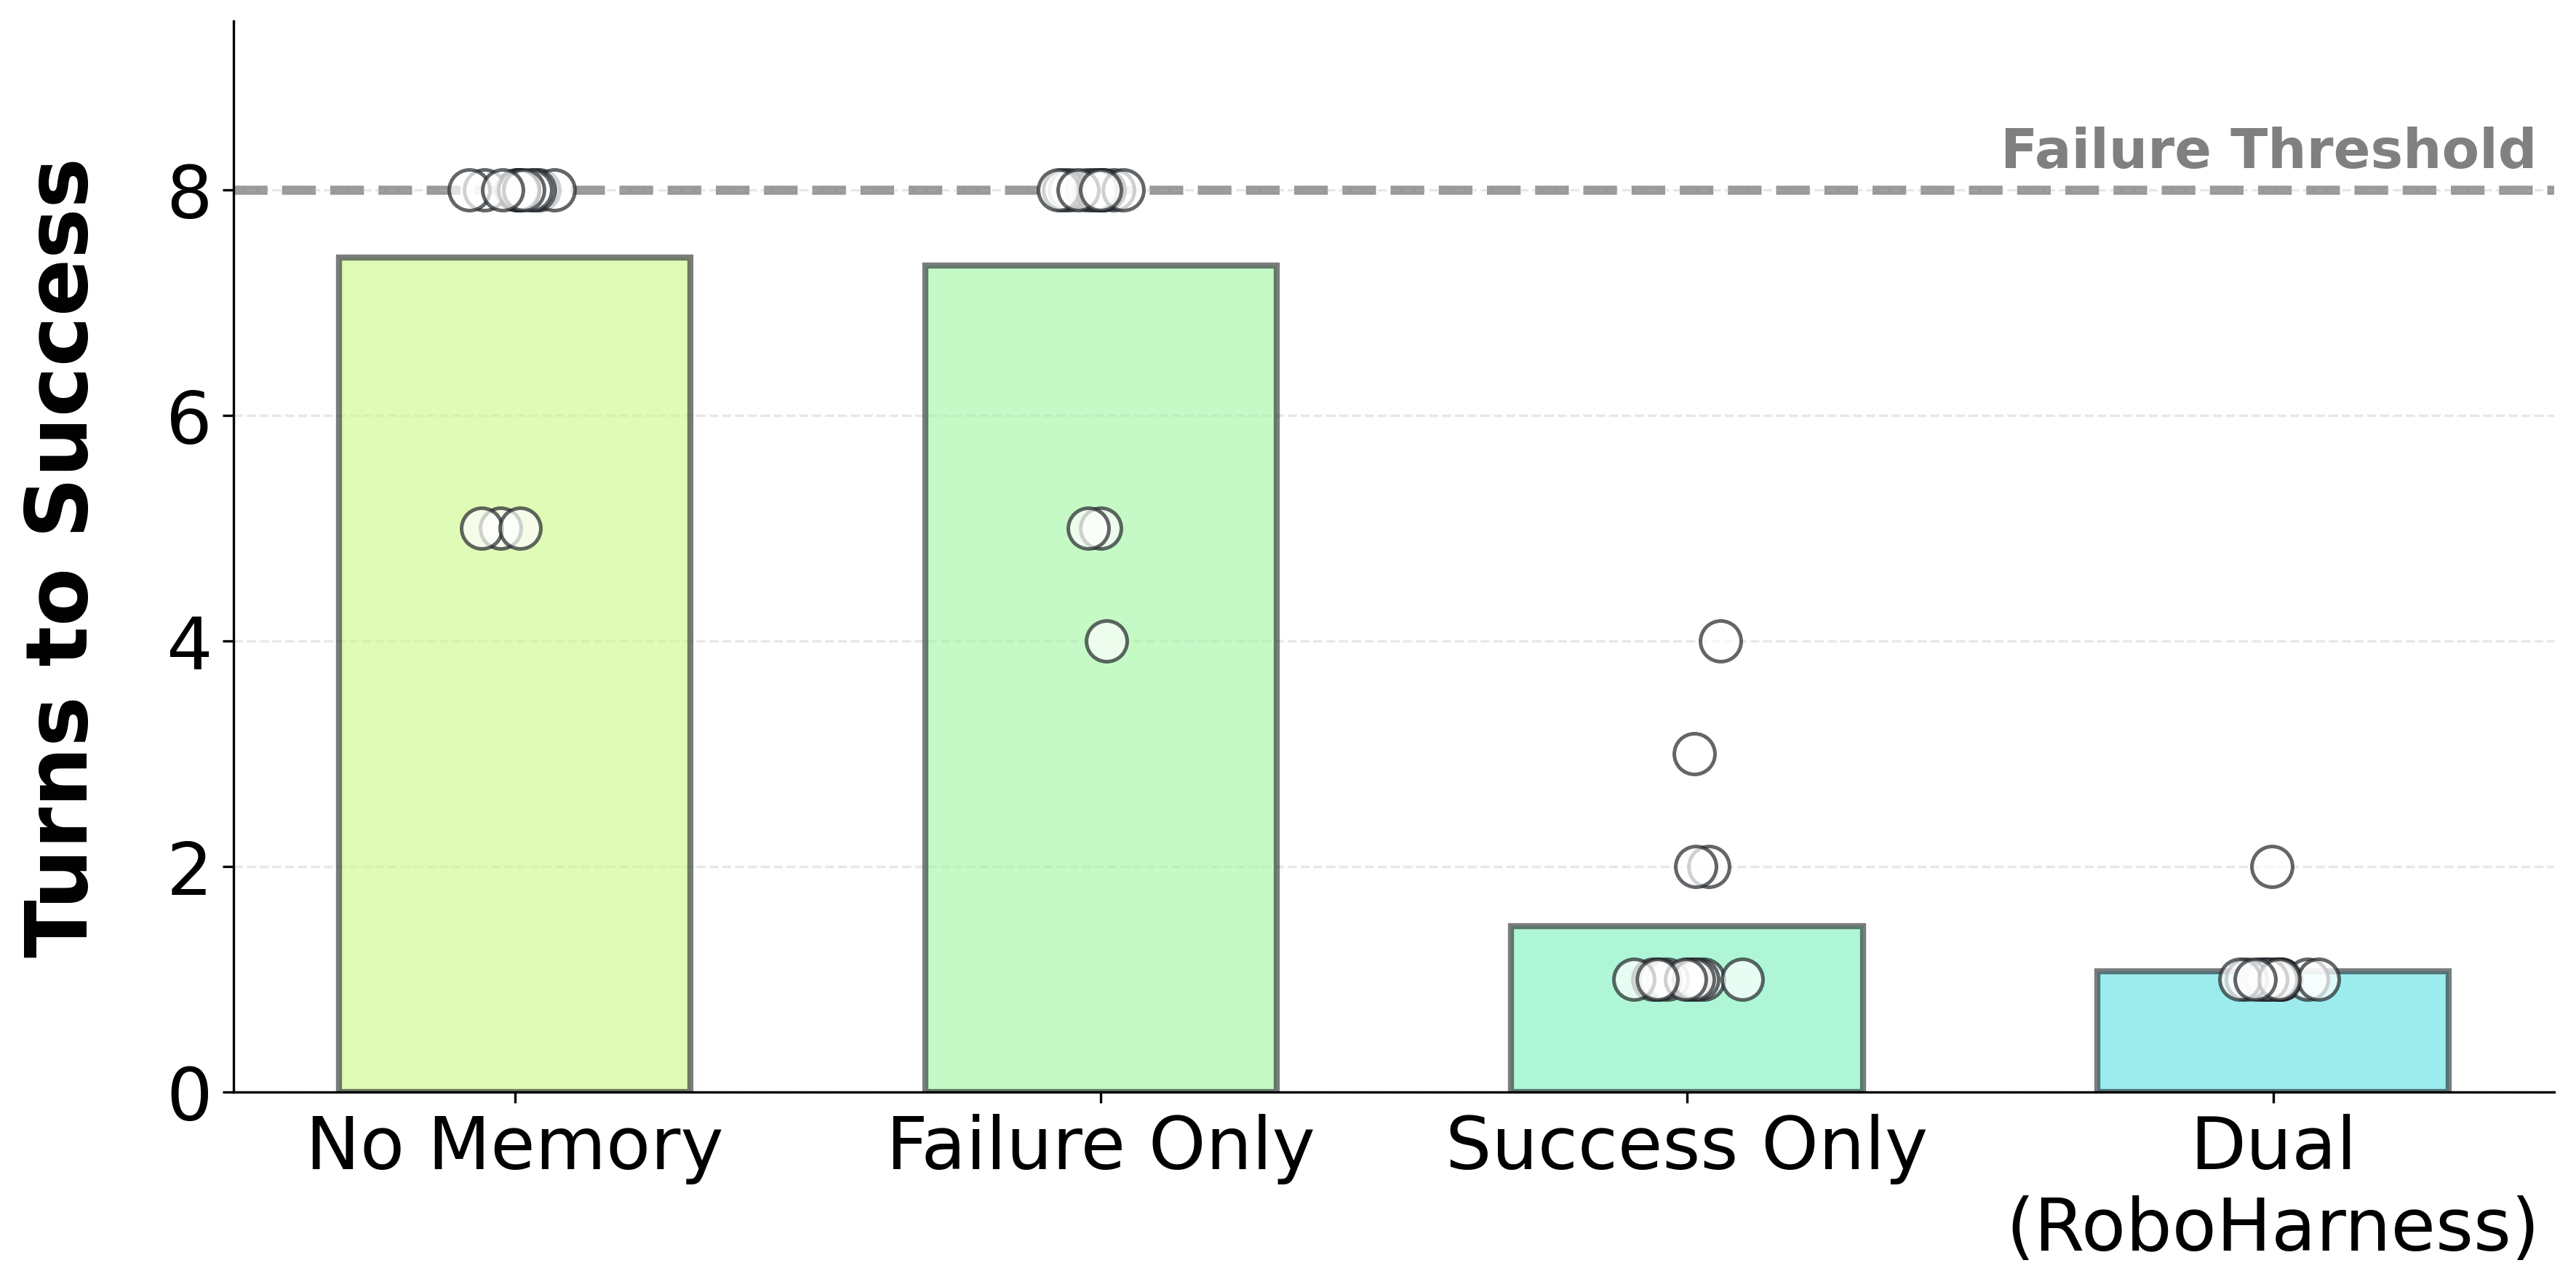
\includegraphics[width=0.4\textwidth]{figure/ablation_dual_memory.png}
    \caption{\textbf{消融实验。}达到目标干预方案所需推理轮数的分布。}
    \label{fig:ablation_beeswarm}
    \vspace{-0.5em}
\end{figure}

如图~\ref{fig:ablation_beeswarm} 所示，无记忆基线始终达到最大执行超时（$Mean=7.40$），表明零样本推理不足以实现 OOD 恢复。
虽然\textit{仅成功}记忆把平均轮数降至 $1.47$，但仍表现出显著的随机方差。
相比之下，\textbf{\sys（双记忆）}收敛到接近最优的\textbf{$1.07$} 轮。
双记忆库约束了视觉--语言编排器的搜索空间，使其能够进行有方向的决策，而非随机探索。

\subsubsection{双阶段记忆巩固的影响}

双记忆库提供原始数据，而这些经验的质量由第~\ref{Evolution} 节所述的迭代归因模块控制。
我们通过三种配置评估这一过程：\textbf{无 RAG}（基线）、\textbf{有限 RAG}（单阶段在线归因）以及\textbf{丰富 RAG}（\sys\ 的双阶段巩固）。

\newcolumntype{M}[1]{>{\centering\arraybackslash}m{#1}}
\renewcommand{\arraystretch}{1.1}
\setlength{\tabcolsep}{3pt}

\begin{table*}[t]
\vspace{0.5em}
\centering
\caption{\textbf{消融实验。}不同 RAG 配置的推理逻辑与成功率比较。}
\label{ablation}
\footnotesize
\begin{tabularx}{\textwidth}{|M{1.8cm}|X|M{3.5cm}|M{2.1cm}|M{1.8cm}|M{1.1cm}|}
\hline
\textbf{RAG 配置} & \multicolumn{1}{c|}{\textbf{通过 RAG 进行的编排器推理}} & \textbf{MCP 工具} & \textbf{动作结果} & \textbf{任务图像} & \textbf{SR（\%）} \\ \hline
\multirow{3}{*}{无 RAG} & 相同纹理导致目标身份存在歧义。 & $o_t' = \text{Paint-to-Action}(o_t, \theta_{\text{dist}})$ & 高亮碗 & \multirow{3}{*}{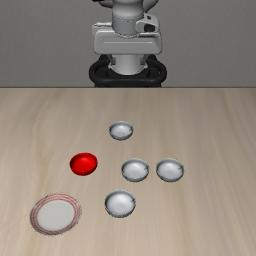
\includegraphics[width=0.95cm, valign=m]{figure/no_origin.jpg}} & \multirow{3}{*}{19.2} \\ \cline{2-4}
 & 盘子阴影可能造成检测错误。 & \texttt{none} & --- & & \\ \cline{2-4}
 & 背景干净，未发现干扰物。 & \texttt{none} & --- & & \\ \hline
\multirow{4}{*}{有限 RAG} & 靠近边缘造成遮挡；高亮目标。 & $o_t' = \text{Paint-to-Action}(o_t, \theta_{\text{dist}})$ & 高亮碗 & \multirow{4}{*}{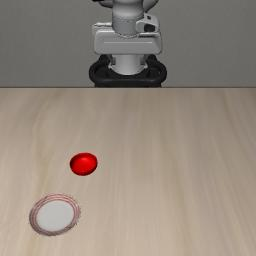
\includegraphics[width=0.95cm, valign=m]{figure/limit_origin.jpg}} & \multirow{4}{*}{48.8} \\ \cline{2-4}
 & 1. \textbf{过往失败}表明误识别风险较高。 & \multirow{2}{*}{$o_t'' = \text{Eraser}(o_t', \theta_{\text{conf}})$} & \multirow{2}{*}{移除 4 个干扰物} & & \\
 & 2. 通过\textbf{移除}相同干扰物来聚焦。 & & & & \\ \cline{2-4}
 & \textbf{替换背景}以减少视觉噪声。 & $o_t''' = \text{Eraser}(o_t'', \theta_{\text{conf}})$ & 替换背景 & & \\ \hline
\multirow{5}{*}{丰富 RAG} & 1. \textbf{失败记忆表明干扰物风险很高}。 & \multirow{4}{*}{$o_t' = \text{Eraser}(o_t, \theta_{\text{conf}})$} & \multirow{4}{*}{移除 4 个干扰物} & \multirow{5}{*}{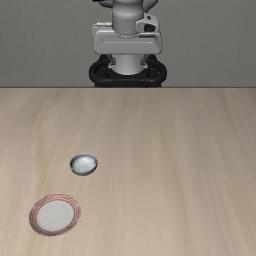
\includegraphics[width=0.95cm, valign=m]{figure/rich_origin.jpg}} & \multirow{5}{*}{60.1} \\
 & 2. \textbf{记忆}要求明确移除每一个碗。 & & & & \\
 & 3. 策略性保留目标和盘子。 & & & & \\
 & 4. 使用精确位置指导策略。 & & & & \\ \cline{2-4}
 & \textbf{已无干扰；无需视觉叠加。} & \texttt{none} & --- & & \\ \hline
\end{tabularx}
\end{table*}

\begin{figure}[htbp]
     \centering
     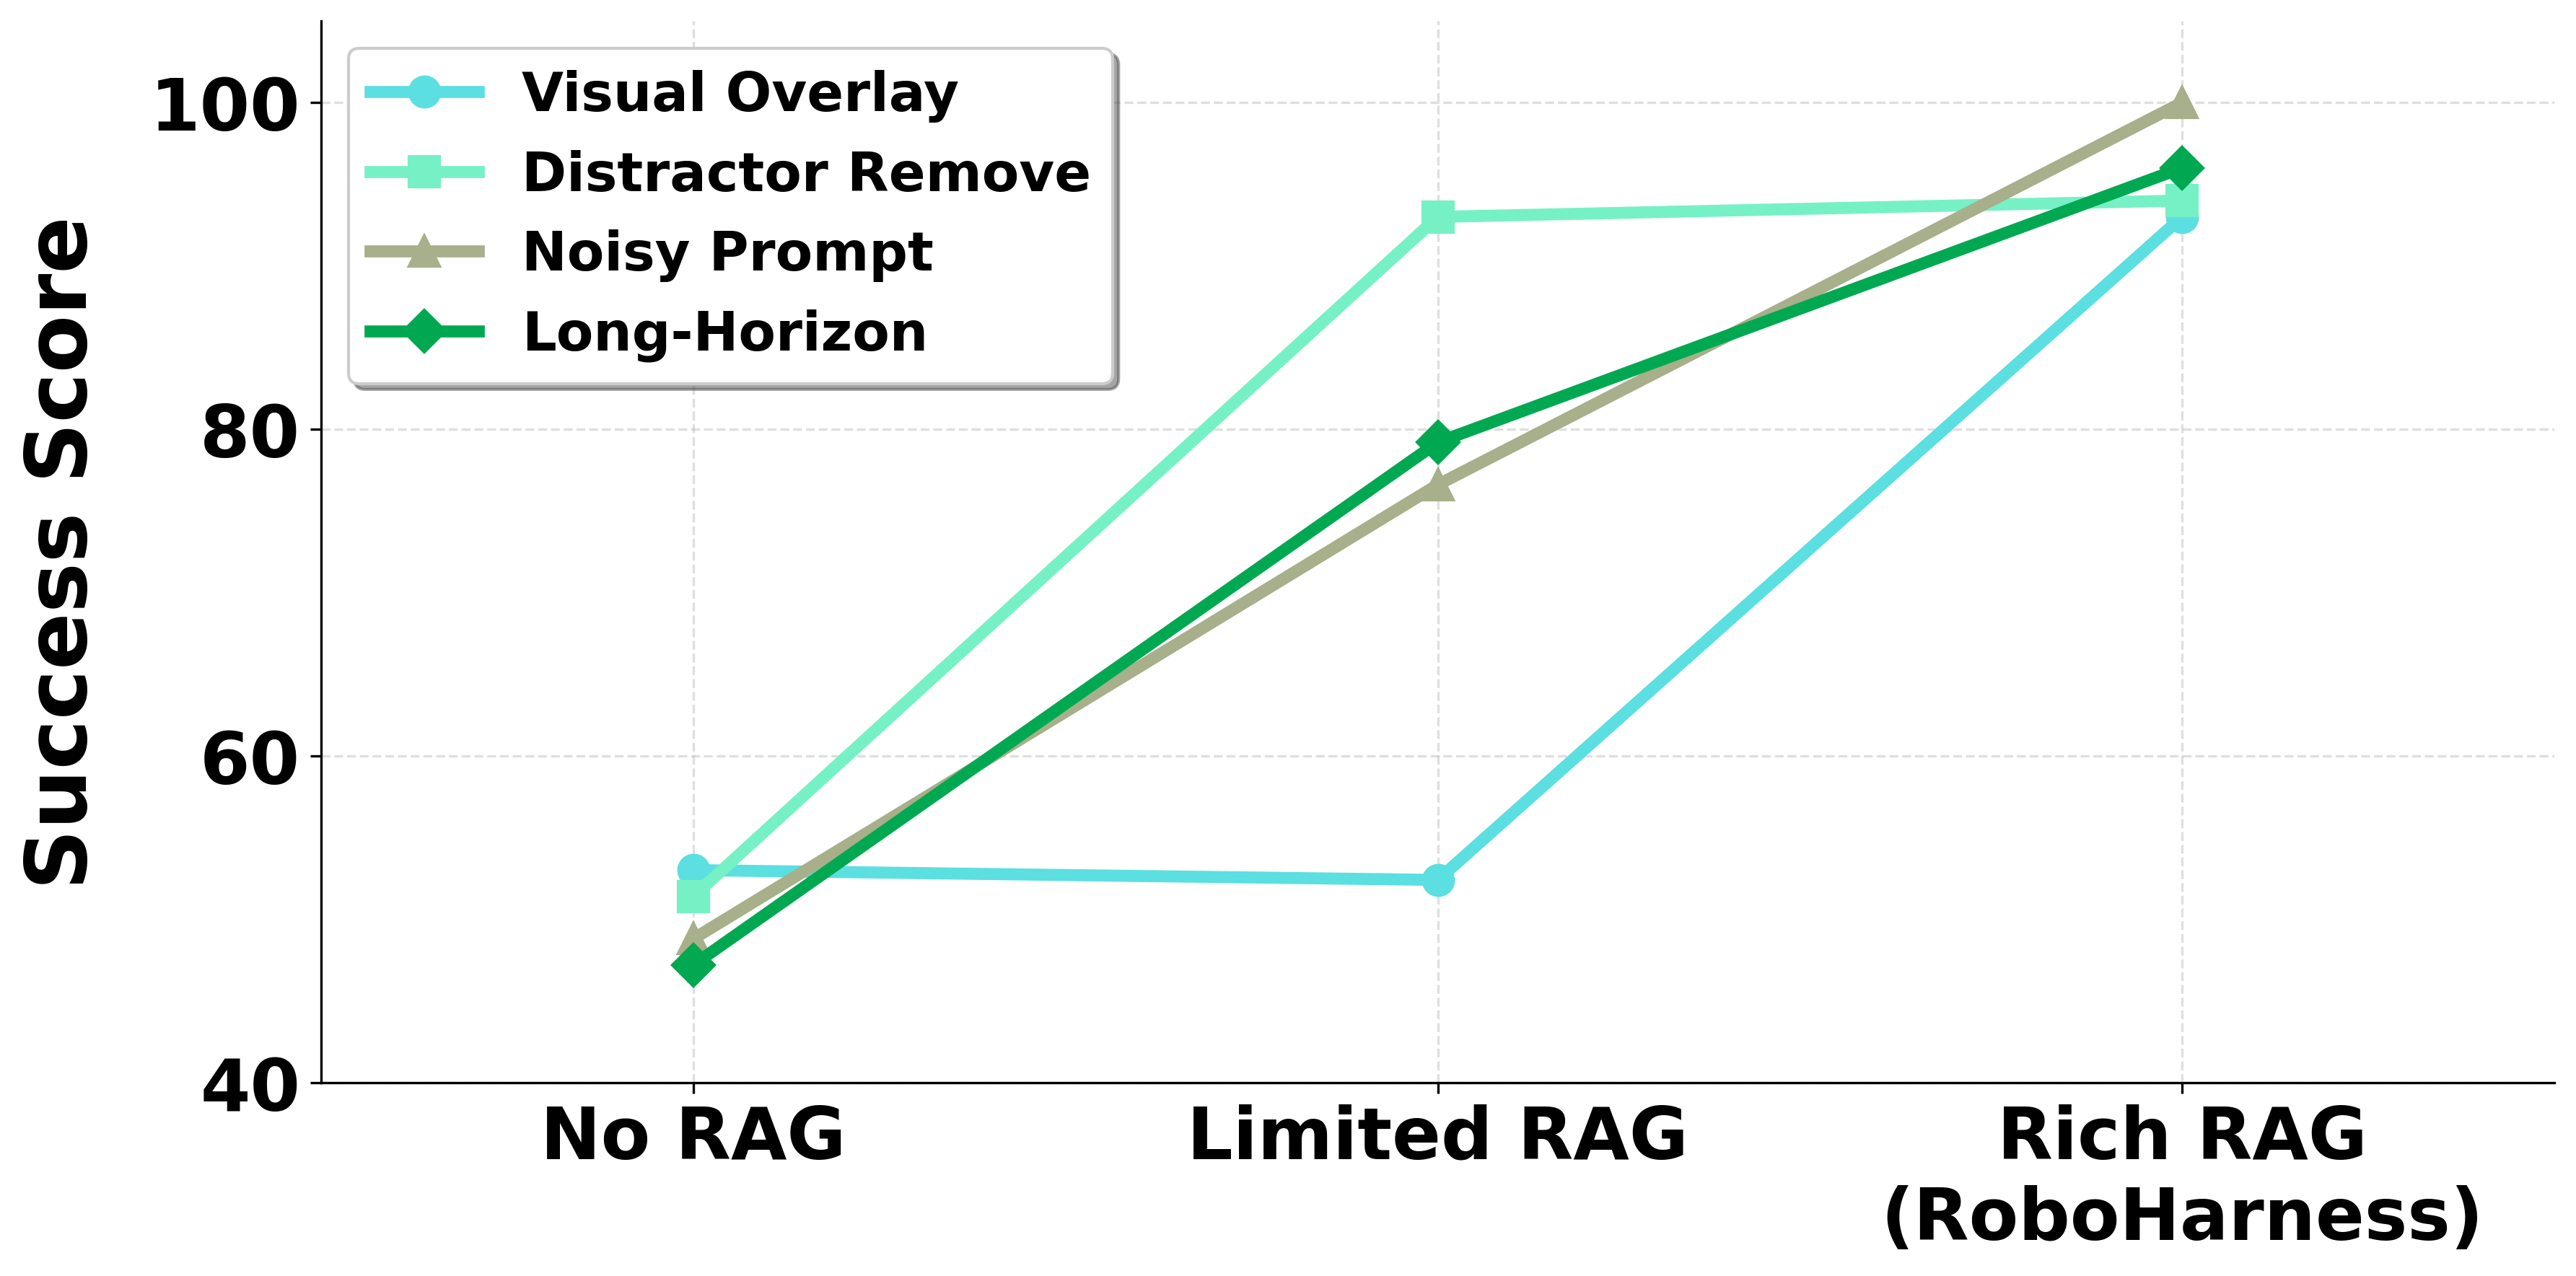
\includegraphics[width=0.4\textwidth]{figure/ablation2.png}
     \caption{\textbf{消融实验。}不同配置下定性推理深度分数的演化。}
     \label{score_qwen}
\end{figure}

\noindent\textbf{推理深度的定性评估。}
我们使用 Qwen3-VL-32B 为所生成指令的逻辑连贯性评分。
如图~\ref{score_qwen} 所示，丰富 RAG 在所有维度上始终取得最高评分。
这一提升来自更聚焦的推理轨迹：它们优先考虑关键干预点并减少无效动作。
这些结果表明，更高质量的 RAG 数据能改善因果理解，形成更鲁棒的工具调用链，与定量提升相一致。

\noindent\textbf{定量性能与稳定性。}
我们使用 $\pi_{0.5}$ 评估一个“杂物移除”变体。
如表~\ref{ablation} 所示，成功率随 RAG 信息丰富度提高。
无 RAG 的成功率仅为 $19.20\%$；与第~\ref{Main Results} 节比较可见，没有 RAG 的编排器指导会因引入负面偏差而适得其反。
有限 RAG 将性能提高到 $48.80\%$，但仍依赖冗余步骤（例如不必要的背景替换）。
丰富 RAG（\sys）使用精简的推理链达到 $60.10\%$，展现出更高的策略效率和精度。

\endinput
